\documentclass[12pt]{article}
\usepackage{ucs}
\usepackage[utf8x]{inputenc}
\usepackage[T1]{fontenc}
\usepackage{lmodern}
\usepackage[english]{babel}
\usepackage[nottoc]{tocbibind}
\usepackage[left=2.5cm,right=2.5cm,top=2.5cm,bottom=2.5cm,]{geometry}
\usepackage{graphicx}
\usepackage{nameref}
\usepackage[hidelinks]{hyperref}
\usepackage{sidecap}
\usepackage{wrapfig}
\usepackage[bottom,hang]{footmisc} 
\usepackage{acronym}
\usepackage{multirow}
\usepackage{color}
\usepackage{capt-of}
\usepackage{array,				%better tables
			tabularx,			%instead of tabular*             
			booktabs,			%tables for good publications
}
\usepackage{afterpage,hyperref} 
\usepackage{listings}
\lstset{
    basicstyle=\ttfamily\footnotesize,
    numbers=left,
    xleftmargin=15pt,
}

\usepackage{subfigure}
%\usepackage{float}


% TabularX column defintions
\newcolumntype{L}[1]{>{\raggedright\let\newline\\\arraybackslash\hspace{0pt}}m{#1}}
\newcolumntype{C}[1]{>{\centering\let\newline\\\arraybackslash\hspace{0pt}}m{#1}}
\newcolumntype{R}[1]{>{\raggedleft\let\newline\\\arraybackslash\hspace{0pt}}m{#1}}

%\captionsetup[table]{aboveskip=4pt}
%\captionsetup[table]{belowskip=0pt}
%\captionsetup{hypcap=false}



%--------------------------MAKETITLE-------------------------------%
\title{Seminar on Privacy in Ubiquitous Computing}
\date{\today}
\author{Mehmed Mustafa, Chris Warin} 

\begin{document}
%--------------------------BEGINNING-------------------------------%
\pagenumbering{roman} 
\maketitle
\thispagestyle{empty}
\begin{abstract}

\end{abstract}

\newpage
\tableofcontents
\newpage

%-----------------------SECTION START------------------------
\pagenumbering{arabic}


%\setcounter{table}{0}

\section{Introduction} \label{sec:Intro}

\section{Foundations} \label{sec:Foundations}

\section{Approach} \label{sec:Approach}

\section{Conclusion} \label{sec:Conclusion}

\section{Template Section} \label{sec:Template}
    This template should give us a first version we can start of with. This last section should support us in writing a more coherent paper together. Therefore I put some guidelines for the writing in section~\ref{sec:Guidelines}. Also there are some example for the use of functionalities in Section~\ref{sec:Examples}. You can copy them and adapt them the way you need them. Just leave this section here for now.


    \subsection{Guidelines} \label{sec:Guidelines}
        \begin{itemize}
        \item \textbf{pushing to the repo} \\
            When you push the newest version to the repo, please leave out the files created by the compiler (besides the pdf). The report on the repo just needs the tex-file, the bib-file and maybe the most current pdf-file. Of course push the changes to the sub folders if you added images or sources.

        \item \textbf{references} \\
            For every section, subsection, figure, or table you include give it a label. Therefore everyone can refer to it later. It can be done by \textit{$\backslash$label\{marker\}}. The marker should declare the type of the object and a short (one word in the best case) name for the object. The types are "sec:" for a section, "fig:" for a figure and 'tab:' for a table. You can refer to them then by \textit{$\backslash$ref\{fig:example\}}. Also you should use a $\sim$ symbol before instead of normal space to avoid line breaks there.

        \item \textbf{citations} \\
            For cititions the BibTex code for the source needs to be in the 'literature\_list.bib' file. You can usually get them pretty easily from \textit{Google Scholar}. Please safe all papers/sources you used in the "sources" folder in addition. The citation can then be made by \textit{$\backslash$cite\{antonopoulos2017mastering\}} for example. Please use the $\sim$ here too. The result then looks like this~\cite{shu2016cardea}.


        \item \textbf{abbreviations} \\
            Please use the $\backslash$ac\{...\} command to handle abbreviations. You can define them at the end of the document. Here is one example... When used the first time it automatically defines the abbreviation: \ac{AI}. For all further times it just prints: \ac{AI}. Also the plural is possible \acp{AI}

        \end{itemize}


    \subsection{Examples} \label{sec:Examples}

    \begin{figure}[t]
        \centering
        \subfigure[Cadrea Overview]{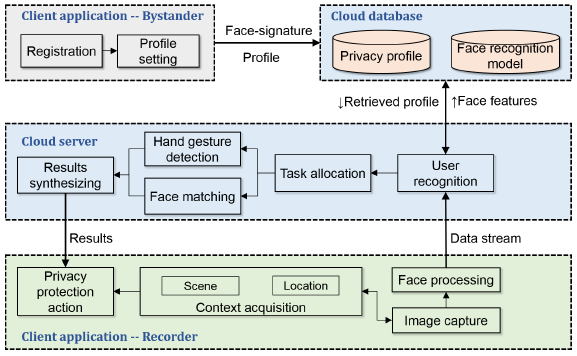
\includegraphics[width=.49\textwidth]{img/cardea_overview_diagram.png}}
        \subfigure[Cadrea Overview]{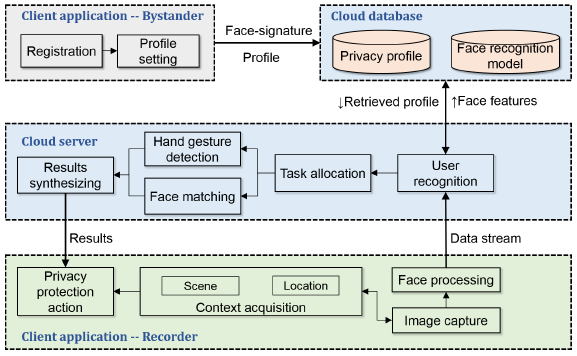
\includegraphics[width=.49\textwidth]{img/cardea_overview_diagram.png}}
        \caption{Example for 2 subfigures.}
        \label{fig:CardeaDiagram}
    \end{figure}



    \begin{figure} [t]
        \centering
        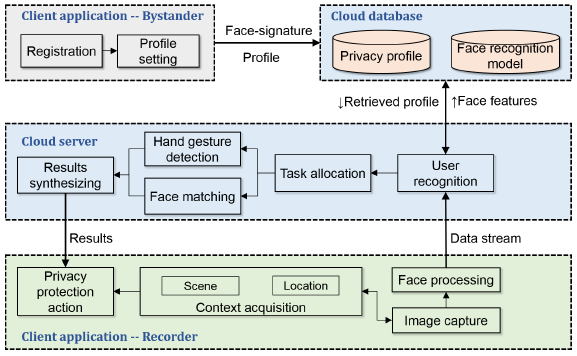
\includegraphics[width=.3\textwidth]{img/cardea_overview_diagram.png}
        \caption{Example for a single figure.}
        \label{fig:drake}
    \end{figure}



    \begin{table}[t]
        \centering
        %\captionof{table}{The tasks for the different prototypes.}
        \begin{tabular}{|C{.07\textwidth}|L{.41\textwidth}|L{.41\textwidth}|}
            \hline & \textbf{SVM} & \textbf{Neural Network} \\
            \hline MR-1 & Permutation of training \& test features & Permutation of input channels (RGB channels) for
training \& test data \\
            \hline MR-2 & Permutation of order of training instances & Permutation of the convolution operation order for
training \& test data \\
            \hline MR-3 & Shifting of training \& test features by a constant (only for RBF kernel) & Normalizing the test data \\
            \hline MR-4 & Linear scaling of the test features (only for linear kernel) & Scaling the test data by a constant \\
            \hline
        \end{tabular}
        
        \captionof{table}{Content totally out of context, literally just as an example for a table.}
        \label{tab:relations}
    \end{table}  

        \begin{center}
    \begin{lstlisting}
    # Computes the hash of the Block
    def compute_hash(self):
        # self.__dict__ -> all variables inside the Block class
        encoded_block = json.dumps(self.__dict__, sort_keys=True)
        return hashlib.sha256(encoded_block).hexdigest()
    \end{lstlisting}
    \end{center}




\newpage

%-------------------References---------------------------%
\section*{Abbreviations and Acronyms}
\addcontentsline{toc}{section}{Abbreviations and Acronyms}
\begin{acronym}[Bash]
\acro{AI} {\textit{Artificial Intelligence}}
\acro{ML} {\textit{Machine Learning}}


\end{acronym}

%----------------List-of-Tables--------------------%
%Comment the following lines out if you dont have tables or figures
\listoftables
\listoffigures
\bibliographystyle{plain}
\bibliography{literature_list}
\end{document}
